\section{Reproducibility Details}
\label{sec:appendix-reproducibility}
\raggedbottom
\makeatletter
\setlength{\@fptop}{0pt}
\setlength{\@fpsep}{12pt plus 2pt minus 2pt}
\setlength{\@fpbot}{0pt plus 1fil}
\setlength{\@dblfptop}{0pt}
\setlength{\@dblfpsep}{12pt plus 2pt minus 2pt}
\setlength{\@dblfpbot}{0pt plus 1fil}
\makeatother

This section records the generation, query-construction, retrieval, and replay
settings needed to reproduce the experiments.

\subsection{Complementary Reference Generation}

We use the following Qwen2.5-7B-Instruct revision for both the model and
tokenizer:

{\footnotesize\noindent\texttt{fe11104b620d588ccc049ff6631dd3ea002e3d98}\par}

The unquantized BF16 model runs with MLX-LM 0.31.2. Decoding uses a
temperature of 0.7, top-$p$ of 0.9, top-$k$ of 20, and a maximum of 256 new
tokens. Queries are sorted by identifier and processed in batches of eight.
Each batch seed is derived from the protocol version, dataset, prompt hash, and
batch index using the first 64 bits of their SHA-256 digest.

\begin{promptbox}{Prompt 1. Complementary Reference Generation}
\textbf{System prompt}

You generate evidence-like reference passages for information retrieval.

Given one search query, return exactly five concise, complementary passages
that could plausibly occur in relevant documents. Preserve every named entity,
relation, number, polarity, temporal condition, scope, and constraint in the
query. Add useful aliases, technical terminology, and paraphrases, but do not
broaden the information need or invent a specific answer. Each passage must be
one sentence of at most 25 words.

Return one single-line JSON array containing exactly five distinct strings.
Count the five array items before responding. Do not output an object key,
query identifier, Markdown, placeholders, or any other text. Every item must
contain a substantive passage.

\par\smallskip\hrule\smallskip
\textbf{User input}\par
\texttt{\{"query":"\{query\}"\}}
\end{promptbox}

The user input is serialized as a canonical JSON object with one
\texttt{query} field.
XGrammar 0.2.1 requires exactly five strings; validation rejects empty,
duplicate, or placeholder passages. Invalid output is retried once with the
same seed and validation feedback, then falls back to the unexpanded query.

The second generator is Mistral-7B-Instruct-v0.3 at revision

{\footnotesize\noindent\texttt{c170c708c41dac9275d15a8fff4eca08d52bab71}.\par}

It uses the same decoding, batching, and validation settings.

\subsection{Query Construction}

Orthogonal residual expansion uses float32 throughout. Shared expansion uses
the same \texttt{query [SEP] reference} representations, but averages and
normalizes them without removing the component parallel to the original query.

For sparse retrieval, the expanded query contains one copy of the original
query followed by the selected reference passages. BM25 scores under the
original and expanded queries are stored separately before applying the
document-wise score product. The binary-mask ablation retains the expanded-query
score only for documents matched by both queries; the references-only ablation
removes the original query. DESA neither repeats the original query nor uses
MuGI's repetition coefficient.

\subsection{Baseline Reproduction}

All generative baselines use the same primary generator. Exact prompts and the
reproduction code are available at
\url{https://github.com/ln-one/hybrid-query-construction}.

HyDE generates eight hypothetical documents per run and averages their
normalized representations; its sparse channel uses the original query. FiQA,
ArguAna, SciFact, and TREC-COVID use task-specific instructions, the remaining
datasets use a general instruction, and generation is capped at 512 new tokens.

Query2doc generates one pseudo-document of at most 120 words. Dense retrieval
encodes it with the original query; sparse retrieval concatenates it with five
copies of the original query.

MuGI generates five pseudo-references. Dense retrieval averages the five
query--reference representations. Sparse retrieval repeats the original query

\[
\left\lfloor\frac{\sum_{i=1}^{n}|r_i|}{|q_o|\beta}\right\rfloor
\]

times before appending all references, where $|\cdot|$ denotes character
length and $\beta=4$. We reproduce MuGI's generation and query integration
components without its pseudo-relevance feedback calibration.

\subsection{Retrieval Implementation}

BGE-small-en-v1.5 uses revision

{\footnotesize\noindent\texttt{5c38ec7c405ec4b44b94cc5a9bb96e735b38267a}.\par}

Queries are prefixed with
``Represent this sentence for searching relevant passages:'' and encoded
with a maximum length of 512 tokens. Contriever uses mean pooling at revision

{\footnotesize\noindent\texttt{2bd46a25019aeea091fd42d1f0fd4801675cf699}.\par}

All query and document embeddings are normalized. Pyserini 2.3.0 runs with
Java 21 and uses \texttt{DefaultEnglishAnalyzer}. A separate Lucene index is
built for each dataset and each TREC-COVID snapshot, so BM25 collection
statistics are computed within the corresponding corpus. Documents with equal
retrieval or fusion scores are ordered by the UTF-8 order of their identifiers.

\subsection{Access-Depth Replay}

This implements the fixed bound-based replay protocol adopted in
Section~\ref{sec:quality-access} from \citet{zhang2026exact}. The replay starts
with empty dense and sparse prefixes. After reading $l_c$
items from channel $c$, its next unread contribution is bounded by

\[
u_c(l_c)=\frac{1}{60+l_c+1}.
\]

The bound becomes zero after exhaustion. The replay reads the channel with the
larger bound, breaking ties toward dense. An observed document's accumulated
score is a lower bound; an unseen contribution is bounded by the corresponding
next-unread value, and a document unseen in both channels by their sum. Replay
stops when these bounds certify top-20 membership and order, recording
$(L_D,L_S)=(l_D,l_S)$.

\subsection{Artifact Traceability}

Generation records store the raw and parsed output, hashes, decoding settings,
seed, retries, runtime lock, and code commit. Query-level records store the
method, generation run, effectiveness, $(L_D,L_S)$, sparse support and
exhaustion, ordered top-20, and hashes of the compressed rankings,
configuration, generation, and replay trace.

The Python environment is fixed by \texttt{uv.lock}; Java is checked before
retrieval. A hash manifest records code, configurations, prompts, inputs,
models, generations, and rankings. Reported tables are rebuilt from the
query-level records.

\section{Operator Properties and Mechanism Diagnostics}
\label{sec:appendix-operators}

\subsection{Properties of the Channel Operators}

For the dense construction, each contextual vector $\mathbf v_i$ is unit
normalized. The triangle inequality gives

\[
\|\bar{\mathbf v}_r\|
\leq \frac{1}{n}\sum_{i=1}^{n}\|\mathbf v_i\|=1.
\]

Orthogonal projection cannot increase the norm, so
$\|\mathbf z\|\leq 1$. Since $\mathbf v_o^\top\mathbf z=0$ and
$\|\mathbf v_o\|=1$,

\[
\begin{aligned}
\mathbf e_D^\top\mathbf v_o
&=\frac{1}{\sqrt{1+\|\mathbf z\|^2}},\\
\angle(\mathbf e_D,\mathbf v_o)
&=\arctan\|\mathbf z\|\leq\frac{\pi}{4}.
\end{aligned}
\]

If $\mathbf z=\mathbf 0$, normalization leaves $\mathbf v_o$ unchanged.

For sparse retrieval, non-negativity gives
$\operatorname{supp}(s_os_r)=
\operatorname{supp}(s_o)\cap\operatorname{supp}(s_r)$. Additivity and the
inclusion of $q_o$ in $q_r$ imply
$\operatorname{supp}(s_o)\subseteq\operatorname{supp}(s_r)$, yielding exact
support preservation. If $s_r=c\,s_o$ for $c>0$, then
$s_A=c\,s_o^2$; squaring is strictly increasing on positive scores, so the
ranking is unchanged. Multiplying $s_o$ or $s_r$ by a positive global constant
only rescales every anchored score and likewise leaves the ranking unchanged.

\subsection{Mechanism Diagnostics}
\label{sec:appendix-mechanism}

Table~\ref{tab:mechanism-diagnostics} reports dense angle, one minus sparse
top-20 overlap with Original, and the mean reciprocal-rank change of judged
relevant documents present in the exported rankings. Macros weight datasets
equally.

\begin{table*}[!t]
\centering
\small
\setlength{\tabcolsep}{5.0pt}
\begin{tabular}{lrrrr}
\toprule
Dataset & Dense angle ($^\circ$) & Sparse top-20 turnover (\%) & Relevant RR change & Support retained (\%) \\
\midrule
SciFact        &  9.38 & 18.88 & .0211 & 100.0000 \\
NFCorpus       & 17.65 & 18.69 & .0147 & 100.0000 \\
TREC-COVID     & 12.99 & 45.37 & .0021 & 100.0000 \\
FiQA           & 13.34 & 33.91 & .0204 & 100.0000 \\
ArguAna        &  4.02 &  8.14 & .0048 & 100.0000 \\
Touch\'e-2020 & 14.40 & 37.07 & .0091 &  99.9999 \\
SCIDOCS        & 12.05 & 20.98 & .0028 & 100.0000 \\
\midrule
Equal-dataset macro & 11.98 & 26.15 & .0107 & 100.0000 \\
\bottomrule
\end{tabular}
\caption{Mechanism diagnostics computed from the frozen query constructions
and rankings. Support retained is the mean per-query--draw fraction of the
original sparse support; the displayed macro rounds to 100.0000\%.}
\label{tab:mechanism-diagnostics}
\end{table*}

Figure~\ref{fig:mechanism-distributions} shows the query-level distributions
behind the aggregate diagnostics. One invalid-generation fallback leaves
11,327 query--draw pairs. Their mean
dense angle is $11.98^\circ$ and the maximum is $27.87^\circ$, below the
analytic $45^\circ$ bound. Sparse anchoring changes 26.15\% of the original
sparse top-20 on average.

\begin{figure}[H]
\centering
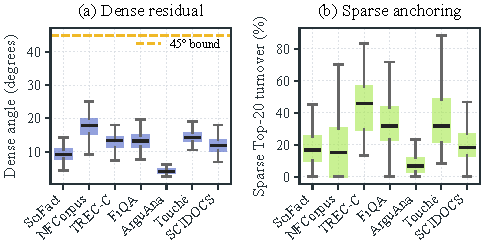
\includegraphics[width=\columnwidth]{figures/fig_mechanism_distributions.pdf}
\caption{Realized behavior of the two channel operators over three generation
draws on seven datasets. Dense angles are measured from the original query;
sparse turnover is one minus top-20 overlap with the original sparse ranking.
Boxes show the interquartile range and median; whiskers extend to 1.5 times the
interquartile range, with outliers omitted.}
\label{fig:mechanism-distributions}
\end{figure}

Within-dataset quartiles show no monotonic relation between either diagnostic
and effectiveness or access depth. Relevant-document reciprocal-rank gain
correlates more strongly with sparse-only nDCG gain than overall turnover does
(.391 versus .078); dense-angle correlations with nDCG gain and depth reduction
are .010 and .011. The data therefore support no angle or turnover threshold.

Exact support preservation assumes a non-negative additive scorer and complete
score export. It holds for six datasets. Touch\'e-2020 omits 25 extremely
low-scoring tail documents across 23 of 147 query--draw pairs; mean and minimum
retention are 99.99990\% and 99.99881\%. We retain these cases and do not call
the Lucene export exactly support preserving there.

\section{Additional Experimental Results}
\label{sec:appendix-analysis}

\subsection{Additional Ablations and Robustness}
\label{sec:additional-results}

Binary masking preserves sparse support but removes original-score magnitude,
lowering macro nDCG@10 by 1.54\% and Recall@20 by 0.74\%. Increasing references
from one to three improves nDCG@10 by 1.91\% and reduces dense/sparse replay
stopping depths by 17.23\%/18.14\%; using five adds 0.35\% nDCG@10 and 0.43\%
Recall@20, with further reductions of 3.83\%/3.40\%.

With Mistral, all four sampled datasets retain non-negative effectiveness
changes and 7.12--47.61\%/7.16--47.62\% dense/sparse depth reductions; 10\% of
sampled ArguAna queries fall back. Contriever improves both metrics on all four
datasets but raises Touch\'e-2020 depths by 14.29\%/4.34\%. Nested TREC-COVID
gains and reductions remain positive but non-monotonic.

\subsection{Matched Operator and QuDAR Controls}

Tables~\ref{tab:operator-controls} and~\ref{tab:qudar-matched} report matched
controls. Operator pairs share references, keep the other channel at Original,
and average three draws within query before inference.

\begin{table*}[!t]
\centering
\footnotesize
\textbf{(a) Per-dataset controlled results}\par\smallskip
\setlength{\tabcolsep}{2.2pt}
\begin{tabular}{llrrrrrrr}
\toprule
Dataset & Method & Queries & nDCG@10 & Recall@20 & $L_D$ & $L_S$ & Sparse support & Exhaust. (\%) \\
\midrule
ArguAna & Original & 1406 & .3941 & .9203 & 157.1 & 156.7 & 8587.8 & 0.00 \\
        & Shared   &      & .4004 & .9265 & 123.4 & 123.0 & 8616.8 & 0.00 \\
        & DESA     &      & .3991 & .9237 & 133.1 & 132.7 & 8587.8 & 0.00 \\
\addlinespace
FiQA & Original & 648 & .3649 & .5260 & 2179.0 & 2076.3 & 28384.6 & 1.23 \\
     & Shared   &     & .3635 & .5391 & 1104.1 & 1103.6 & 46673.3 & 0.00 \\
     & DESA     &     & .3780 & .5450 & 1096.2 & 1065.6 & 28384.6 & 0.93 \\
\addlinespace
NFCorpus & Original & 323 & .3670 & .2099 & 474.4 & 173.7 & 561.5 & 48.61 \\
         & Shared   &     & .3780 & .2260 & 359.1 & 357.6 & 3211.6 & 1.14 \\
         & DESA     &     & .3793 & .2195 & 403.1 & 133.5 & 561.5 & 46.75 \\
\addlinespace
SCIDOCS & Original & 1000 & .1923 & .2721 & 694.8 & 599.3 & 11503.0 & 2.70 \\
        & Shared   &      & .1905 & .2790 & 372.7 & 372.2 & 23239.6 & 0.00 \\
        & DESA     &      & .1940 & .2787 & 448.8 & 387.2 & 11503.0 & 1.63 \\
\addlinespace
SciFact & Original & 300 & .7253 & .9036 & 409.1 & 368.6 & 2765.7 & 4.33 \\
        & Shared   &     & .7325 & .9182 & 284.1 & 282.6 & 4489.0 & 0.33 \\
        & DESA     &     & .7427 & .9200 & 318.3 & 291.6 & 2765.7 & 3.89 \\
\addlinespace
TREC-COVID & Original & 50 & .7781 & .0398 & 6270.9 & 4729.9 & 92683.8 & 2.00 \\
           & Shared   &    & .8169 & .0433 & 787.3 & 786.9 & 141483.1 & 0.00 \\
           & DESA     &    & .8224 & .0435 & 1574.8 & 1574.4 & 92683.8 & 0.00 \\
\addlinespace
Touch\'e-2020 & Original & 49 & .3786 & .3382 & 2081.8 & 2081.4 & 151619.0 & 0.00 \\
              & Shared   &    & .3883 & .3344 & 1221.5 & 1221.3 & 284677.0 & 0.00 \\
              & DESA     &    & .4071 & .3560 & 1127.8 & 1127.4 & 151618.9 & 0.00 \\
\bottomrule
\end{tabular}

\medskip
\begin{minipage}[t]{0.49\textwidth}
\centering
\textbf{(b) Primary statistical tests}\par\smallskip
\setlength{\tabcolsep}{1.2pt}
\begin{tabular}{lll}
\toprule
Comparison / outcome & Effect [95\% CI] & $p/p_{\mathrm{Holm}}$ \\
\midrule
Original / nDCG@10   & .0175 [.0111, .0238]    & .0001 / .0004 \\
Original / Recall@20 & .0109 [.0070, .0151]    & .0001 / .0004 \\
Original / $L_D$     & 1023.6 [377.5, 2012.6]  & .0001 / .0004 \\
Original / $L_S$     & 781.9 [356.1, 1339.7]   & .0001 / .0004 \\
\addlinespace
Shared / nDCG@10     & .0075 [.0036, .0116]     & .0003 / .0012 \\
Shared / Recall@20   & .0028 [-.0003, .0061]    & .0912 / .2736 \\
Shared / $L_D$       & -121.4 [-367.0, 39.7]    & .3157 / .6313 \\
Shared / $L_S$       & -66.5 [-310.6, 93.0]     & .7909 / .7909 \\
\bottomrule
\end{tabular}
\end{minipage}\hfill
\begin{minipage}[t]{0.49\textwidth}
\centering
\textbf{(c) Fixed-cutoff diagnostics}\par\smallskip
\setlength{\tabcolsep}{2.2pt}
\begin{tabular}{rrrrrr}
\toprule
$L$ & Exact top-20 & \multicolumn{2}{c}{nDCG (\%)} & \multicolumn{2}{c}{Recall (\%)} \\
 & (\%) & Change & Reverse & Change & Reverse \\
\midrule
20   & 1.92 & 18.23 & 8.84 & 22.50 & 3.84 \\
50   & 16.54 & 6.95 & 3.07 & 18.84 & 3.06 \\
100  & 47.40 & 2.17 & 0.73 & 11.74 & 0.99 \\
1000 & 92.62 & 0.19 & 0.01 & 1.18 & 0.00 \\
\bottomrule
\end{tabular}
\end{minipage}
\caption{Additional results. (a) Dataset-level controlled results. (b)
Stratified paired tests after within-query averaging over three generation
draws. (c) DESA query--draw sensitivity to fixed top-$L$, macro-averaged with
equal dataset weight; exact top-20 compares with complete-list fusion, and the
conclusion columns compare DESA with Original.}
\label{tab:per-dataset-controlled}
\label{tab:primary-tests}
\label{tab:cutoff-query-diagnostics}
\end{table*}

\begin{table}[H]
\centering
\scriptsize
\setlength{\tabcolsep}{2.8pt}
\begin{tabular}{@{}lrr@{}}
\toprule
Construction & nDCG@10 & Recall@20 \\
\midrule
Original          & .4572 & .4586 \\
Contextual Dense  & .4622 & .4637 \\
Residual Dense    & .4621 & .4637 \\
Rewrite Sparse    & .4686 & .4670 \\
Product Sparse    & .4714 & .4678 \\
\midrule
\multicolumn{3}{l}{Paired effect (proposed $-$ control)} \\
Dense residual, nDCG   & \multicolumn{2}{l}{$-.00005$ [$-.00086,.00082$], $p_{\mathrm{Holm}}=1.0$} \\
Dense residual, Recall & \multicolumn{2}{l}{$-.00006$ [$-.00043,.00033$], $p_{\mathrm{Holm}}=1.0$} \\
Sparse product, nDCG   & \multicolumn{2}{l}{$ .00283$ [$-.00126,.00693$], $p_{\mathrm{Holm}}=.3650$} \\
Sparse product, Recall & \multicolumn{2}{l}{$ .00078$ [$-.00184,.00331$], $p_{\mathrm{Holm}}=.5689$} \\
\bottomrule
\end{tabular}
\caption{Macro operator controls and query-level paired effects. Holm
correction covers nDCG and Recall within each control pair.}
\label{tab:operator-controls}
\end{table}

\begin{table}[H]
\centering
\scriptsize
\setlength{\tabcolsep}{2.9pt}
\begin{tabular}{lrrrr}
\toprule
Dataset & \multicolumn{2}{c}{nDCG@10} & \multicolumn{2}{c}{Recall@20} \\
 & DESA & QuDAR & DESA & QuDAR \\
\midrule
ArguAna        & .3991 & .3985 & .9237 & .9253 \\
FiQA           & .3780 & .3833 & .5450 & .5554 \\
NFCorpus       & .3793 & .3780 & .2195 & .2227 \\
SCIDOCS        & .1940 & .1957 & .2787 & .2811 \\
SciFact        & .7427 & .7403 & .9200 & .9211 \\
TREC-COVID     & .8224 & .8233 & .0435 & .0438 \\
Touch\'e-2020 & .4071 & .4137 & .3560 & .3500 \\
\midrule
Equal-dataset macro & .4747 & .4761 & .4695 & .4714 \\
\bottomrule
\end{tabular}
\caption{Matched-reference comparison with QuDAR-simple RRF (top-1000
original-sparse (OS), expanded-sparse (ES), original-dense (OD), and
expanded-dense (ED) rankings; $k=60$). DESA--QuDAR paired effects are $-.00145$
[$-.00478,.00181$] for nDCG and $-.00188$ [$-.00400,.00019$] for Recall
($p_{\mathrm{Holm}}=.3966$ and $.1668$).}
\label{tab:qudar-matched}
\end{table}
